\documentclass[11pt]{article}
\usepackage{graphicx}
\usepackage{float}
\usepackage{amsmath}
\usepackage{amsfonts}
\usepackage{multicol}
\usepackage{pdfpages}
\usepackage[backend=biber]{biblatex}
\bibliography{theoretical-framework.bib}
\usepackage[bindingoffset=0.0in,%
            left=2.0cm,right=2.0cm,top=2.0cm,bottom=2.0cm,%
            voffset=0in,footskip=1.0cm]{geometry}
\usepackage{titling}


%\setlength{\intextsep}{1.5pt}
%\setlength{\textfloatsep}{-1in}

\begin{document}

%\newgeometry{margin=1in}

\begin{titlepage}
	\centering
	{\scshape\Large \par}
	\vspace{3.5cm}
	{\huge\bfseries A theoretical framework for Attention\par}
	\vspace{1cm}
	{\itshape~Erik de Godoy Perillo\par}% chtex 6
    {\itshape~Advisor: Profa. Dra. Esther Luna Colombini\par}% chtex 6
	\vspace{0.5cm}
	\vfill
	State University of Campinas
	\vfill
	{\large \today\par}
\end{titlepage}

\newpage



%\begin{multicols}{2}

\section{Introduction}
In this document, we briefly formulate a theoretical framework for the concept of Attention.
This framework consists of two main parts:
\begin{itemize}
    \item A \emph{definition} of Attention in terms of its functionalities;
    \item A \emph{model} of Attention.
\end{itemize}
Note that the first element aims at answering the question ``\emph{What} is Attention?''
while the second aims at explaining \emph{how} Attention emerges.

\section{A definition of Attention}
\label{sec:definition}
In this definition, we define a set of \emph{entities of interest} and the phenomenon of Attention in terms of
its \emph{functionalities} and how it relates to the entities.

\subsection{Why is our definition good?}
We believe our definition encompasses what we generally (and intuitively) refer to as attention while being not too broad.
Also, the definition is given in terms related to Computer Science so it’s functionality nicely translates to the domain,
which is important since we (so far) intend to develop AI using computers as we know it today.
We may not encompass every aspect of Attention and even be conflicting with other definitions.
However, this is the set of postulates that we think is the most precise and useful and thus this is
what we choose to use for future work to be based on.

\subsection{Entities}
Below is the list of entities --- or ``terms'' --- we use in this work, along with a brief discussion of the meaning
we give to each term in the context of this work.

\begin{itemize}
    \item\textbf{Data:} information, stimuli. It may be internal or external. Examples: visual information, audio, memories.
    \item\textbf{Program:} algorithm, sequence of computer (or mental) operations. Programs use data as input in order to carry out a sequence of operations that produces output data and/or actions.
    \item\textbf{Process:} the execution of a program on a specific data instance.
    \item\textbf{Computer:} the executor of processes, the “brain”.
    \item\textbf{Resource:} when not specified, we mean “computational resources”, e.g. CPU time.
    \item\textbf{Time:} the flow of time.
    \item\textbf{World:} the external environment.
    \item\textbf{Agent:} the actor in the world.
    \item\textbf{Actions:} the interaction of the agent with the world.
    \item\textbf{Goals:} the ends, objectives to be met.
\end{itemize}

\subsection{What is Attention?}
\emph{Data}, \emph{programs} and \emph{processes} are virtually \emph{infinite}.
Computational \emph{resources} and \emph{actions} are finite.
\emph{Attention} is \emph{the system of allocating resources to processes}.
In other words, \emph{attention} is the entity in \emph{agents} that, given \emph{context} and a set of \emph{processes},
\emph{allocates} \emph{resources} to execute each of them in order to \emph{produce} \emph{outputs} in form of \emph{data} and \emph{actions} in a \emph{correct sequential manner} and in \emph{sensible time} in order to reach \emph{goals}.

\section{How does Attention happen?}\label{sec:taxonomy}
As mentioned in Section~\ref{sec:definition},
in this work we summarize Attention as \emph{the allocation of computing resources to processes}.
Thus, when attention is taking place, the system is performing a \emph{selection process}: it is directing its \emph{computing time budget} to certain \emph{programs} which,
in turn, are being run with some subset of the possible \emph{data} as input.

In some instances, some of the entities may not be subject to such selection, thus remaining fixed.
There may be, for example, systems in which the program to be run and the computing resources are fixed and attention's role
is to just select which data to be used.
Another example is when both the program and the input data are fixed and Attention selects how much computation time
should be dedicated to the process at a given time window.

\begin{figure}[H]
    \centering
    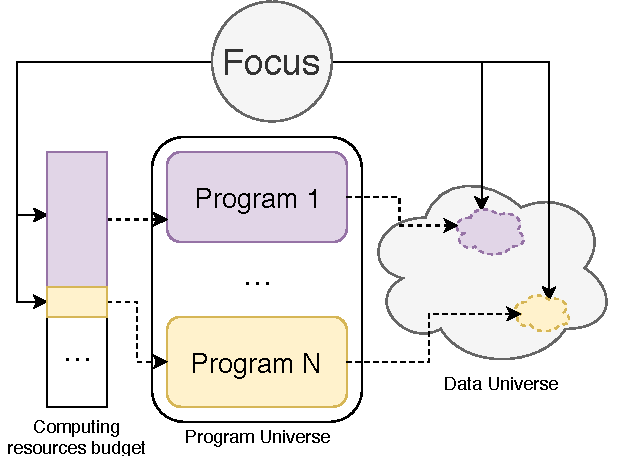
\includegraphics[width=0.7\linewidth]{./img/mind.pdf}\label{fig:mind}
    \caption{High level overview of the focus phenomenon. Attention is responsible for selecting computation resources for programs and also data to be used by the programs.}
\end{figure}

The attention process takes place \emph{along the course of time}.
At each time step in the process, \emph{inputs} of different classes are used to produce a certain \emph{output}.
In a given \emph{timeframe}, the sequence of processing steps produce the emergence of a \emph{selection flow}, or a process.
In this section, we approach the entities and taxonomy related to the \emph{end-to-end} process itself.
In the next section, we specifically model processing at each time step so that the processes described in this section emerge.

\begin{figure}[H]
    \centering
    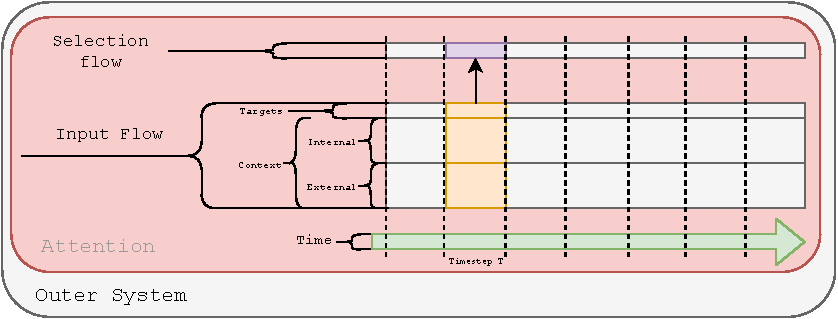
\includegraphics[width=1.0\linewidth]{./img/att_flow.pdf}\label{fig:attflow}
    \caption{The process of Attention.}
\end{figure}

\subsubsection{Types of Inputs}
The information to be used by attention may be classified as either
\emph{context} or \emph{targets}.
Targets are the subjects of selection by attention.
Context is the information used by attention
in order to perform the selection.
Context can be either \emph{internal} (agent state) or \emph{external}
(information about the world) and the context may contain information
about the past.
An example is an recurrent attentional module for focusing on
regions of a video flow. In such case, the hidden state of the network can
be considered internal context; the frames can be considered the
external context and the pixels of the image are the targets.

\subsection{Selection taxonomy}
\subsubsection{Subjects}
The subject of the focus (i.e.\ the target type) may be 1) \emph{data},
2) \emph{computing resources} or 3) \emph{programs}.

For example, in a computer vision task of performing classification on an image,
the data is the input image, the program is
the classification algorithm and the computing resources are the
amount of computation (either time or other measure) that will be applied
to the task of classifying a subset of the image.

Selection of \emph{data} regards selecting targets that are to be used as input
to other processes.
We can further classify this selection based on the nature of the data being
selected, such as:
\begin{itemize}
    \item \textbf{Feature-based}: based on the features of a stimuli, such as color, orientation\ellipsis\
    \item \textbf{Location-based}: based on the location of the stimuli, such as the coordinates of a pixel.
\end{itemize}
Selection of data is the most common of selection nowadays in
Deep Learning systems.
An example of a process of selection of data
is the selection of a window of the input image to be processed
in an image classification task.
In this case, selection can be considered to be location-based.

Selection of \emph{computing resources} is the selection of the amount
of computation to be used for a given process
One example is a recurrent neural network that performs substeps at
each time step and at each step decides how many substeps to perform.

\subsubsection{Continuity}
The continuity of the process may be even 1) \emph{hard} or 2) \emph{soft}.
This division has been popular in Deep Learning research lately.

For \emph{hard} attention, the selection is discrete:
the process performs selection of a subset of the targets.
In the case of data, one example of hard selection is the
selection of a specific subset of $k$ feature vectors (from $m \ge k$ options)
to be further processed.

For \emph{soft} attention, the selection is continuously spread accross the
targets. It can be seen as of type of `weighting'' spread accross the targets.
Using the example above, the selection of feature vectors could be soft ---
in this case, instead of selecting a subset of vectors, every vector
could be given a weight $0 \le w \le 1$ for a further convex combination
of the vectors.

\subsubsection{Flow}
The flow of selection along time in a process
can be classified as 1) \emph{Ephemeral} or 2) \emph{Enduring}.

Ephemeral refers to selection of subjects in the context of a short time window.
For example, in a task of visual control of a car,
an attention process to identify the abrupt appearance of moving obstacles
could be considered ephemeral since it does not take into account
much context.
On the other hand, an attentional process that keeps focus on
a part of the road is not ephemeral, since it's long-termed.

Enduring refers to selection of objects on a long time window.
Using the example above, focusing on the road would be considered
an enduring process.
The enduring focus can be further classified as:
\begin{itemize}
    \item \textbf{Oriented}: An arbitrary focus sequence so as to complete a certain task.
    \item \textbf{Sustained}: Focus restrained to a subset of the targets.
    \item \textbf{Divided}: Focus alternating among a subset of the targets.
\end{itemize}


\begin{figure}[H]
    \centering
    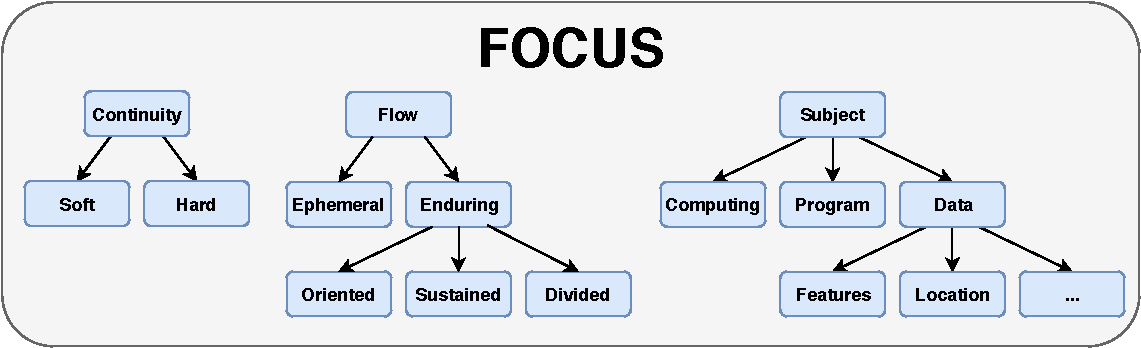
\includegraphics[width=1.0\linewidth]{./img/taxonomy.pdf}\label{fig:taxonomy}
    \caption{Attention attributes.}
\end{figure}

%\subsection{Using the result of attention}
%The result of selections made by attention
%may be used for the allocation of some resource in various ways, such as:
%
%\begin{itemize}
%    \item Choosing the \textbf{amount} of \textbf{computation time} to be used at a certain step;
%    \item Choosing a \textbf{subset} of \textbf{elements} to carry out further computations;
%    \item \textbf{Weighting elements} to perform a certain computation.
%\end{itemize}

\section{Attentional Module}
We propose that the process of Attention --- as discussed in Section~\ref{sec:taxonomy}  --- can emerge by means of \emph{a series of components} --- which we call \emph{attentional modules}. These modules can alter data being processed and the execution flow of the algorithm and provide the functionalities of Attention.

\begin{figure}[H]
    \centering
    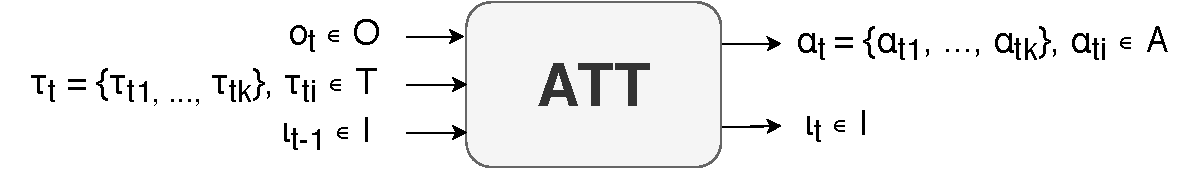
\includegraphics[width=0.9\linewidth]{./img/alt_att_block.pdf}\label{fig:attmodule}
    \caption{Attentional module.}
\end{figure}

Figure~\ref{fig:attmodule} illustrates the attentional module. At each time step $t$, the module receives as \emph{input}:
\begin{itemize}
    \item Current \emph{outer state} $o_t \in O$, where $O$ is the \emph{outer state set}.
    \item Group of \emph{focus targets} $\tau_t = \{\tau_{t1}, \ldots, \tau_{tk}\}, \tau_{ti} \in T$,
        where $T$ is the \emph{focus target set}.
    \item Past \emph{inner state} $\iota_{t-1} \in I$, where $I$ is the \emph{inner state set}.
\end{itemize}

The module produces as \emph{output} (as a function of both inputs):
\begin{itemize}
    \item Current \emph{inner state} $\iota_t \in I$.
    \item Current \emph{focus output} $\alpha_t = \{\alpha_{t1}, \ldots, \alpha_{tk}\}, \alpha_{ti} \in A$,
        where $A$ is the \emph{focus output set}.
\end{itemize}

The focus output is the main element of the module: it can be used to allocate \emph{finite resources} to a set of ``candidate targets'' by giving them an ``importance score'' which can be used in any arbitrary way in following steps.
Each element $\alpha_{tk}$ is respective to a target element $\tau_{tk}$.

\subsection{Modules forming an attentional system}
A system with Attention may contain more than one attentional modules --- even in a recursive manner.
Together, these modules always perform the function to provide focus
as discussed in Section~\ref{sec:taxonomy}.
We now provide some examples of how the attentional modules can act to provide such functionalities.

\subsubsection{Soft and Hard focus}
The different focus continuities can be obtained by means of attentional modules in the following manner:
\begin{itemize}
    \item \textbf{Soft Focus}:
        $A = [0, 1]$, with $0 \le \sum_{i=1}^{k} \alpha_{ti} \le 1$
    \item \textbf{Hard Focus}:
        $A = \{0, 1\}$, with $0 \le \sum_{i=1}^{k} \alpha_{ti} \le M$ and $0 \le M \le |\tau_t|$
\end{itemize}

\subsubsection{Example of an entire system}
Figure~\ref{fig:attsystem} shows the diagram of a possible system with attention.
The module \emph{TaskATT} uses hard attention to select a certain task $k$ to be executed for some time at time step $t$.
Among the computations of task $k$, there is the module \emph{DataATT}, which uses soft attention to allocate resources to a set of items.
It is worth noting that time is relative to each attentional module: \emph{TaskATT} has a temporal course over time steps $t$ that is different from that of \emph{DataATT}, which is over time steps $t'$.
Also, their sets of inputs and outputs may differ.
Together, these modules provide two types of focus:
\emph{hard}, \emph{enduring}/\emph{oriented} focus on \emph{programs} and
\emph{soft}, \emph{ephemeral} focus on data.

\begin{figure}[H]
    \centering
    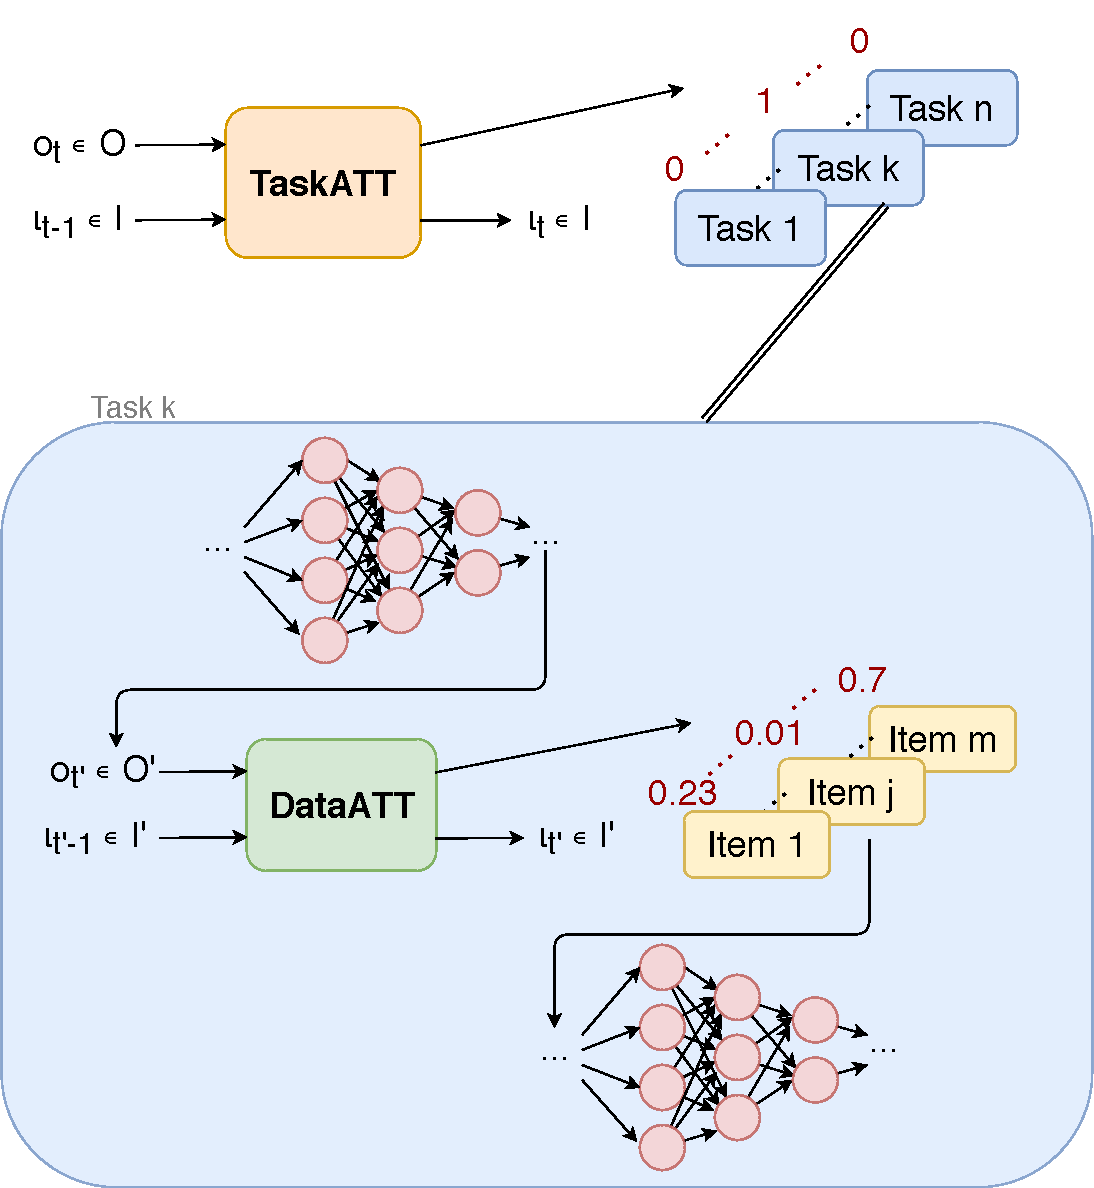
\includegraphics[width=0.7\linewidth]{./img/att_blocks_example.pdf}\label{fig:attsystem}
    \caption{Example of a system that uses attention.}
\end{figure}

\section{Validating the framework}
In this section, we investigate some recent works on attention and see how they fit in our framework.

\subsection{Image Caption Generation}
The work~\cite{ref:show-attend-tell} is among the first to propose using
attention to image caption generation: the encoding of the input image is
represented as a set of vectors --- each respective to a certain spatial region of the image ---
and the attentional component gives weights to each vector at each step in order to produce another
vector to be used in further computations.

\begin{figure}[H]
    \centering
    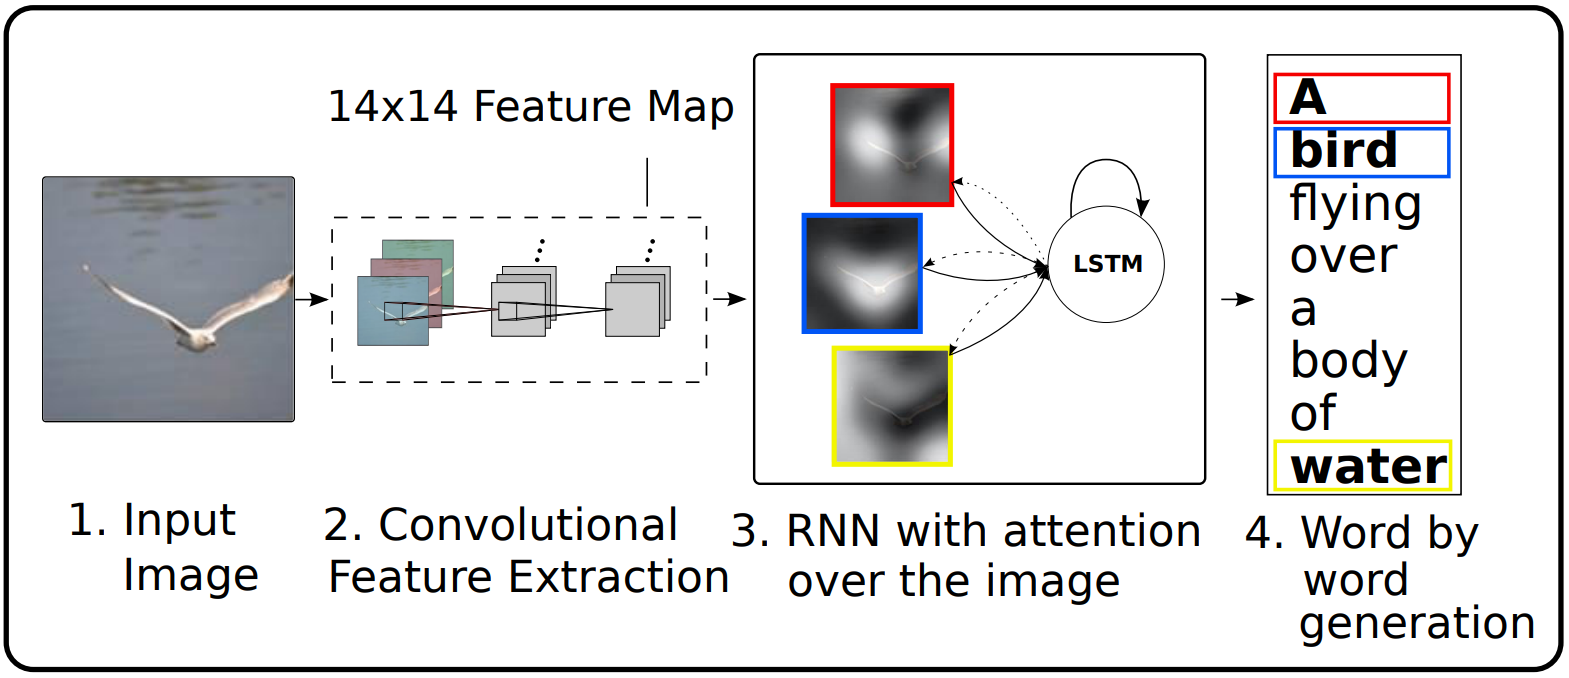
\includegraphics[width=0.8\linewidth]{./img/img_captioning.png}\label{fig:imgcaptioning}
    \caption{Diagram of natural language image description using Attention
    (from~\cite{ref:img-captioning}).}
\end{figure}

While there are many abstract processing substeps in the process, the \emph{end-to-end} effect is that of
a focus with \emph{soft} continuity, with \emph{enduring} and \emph{orienting} flow, targetting \emph{data}
on a \emph{Location-based} manner. Figure~\ref{fig:imgcaptioning} illustrates the proposed model.

\begin{figure}[H]
    \centering
    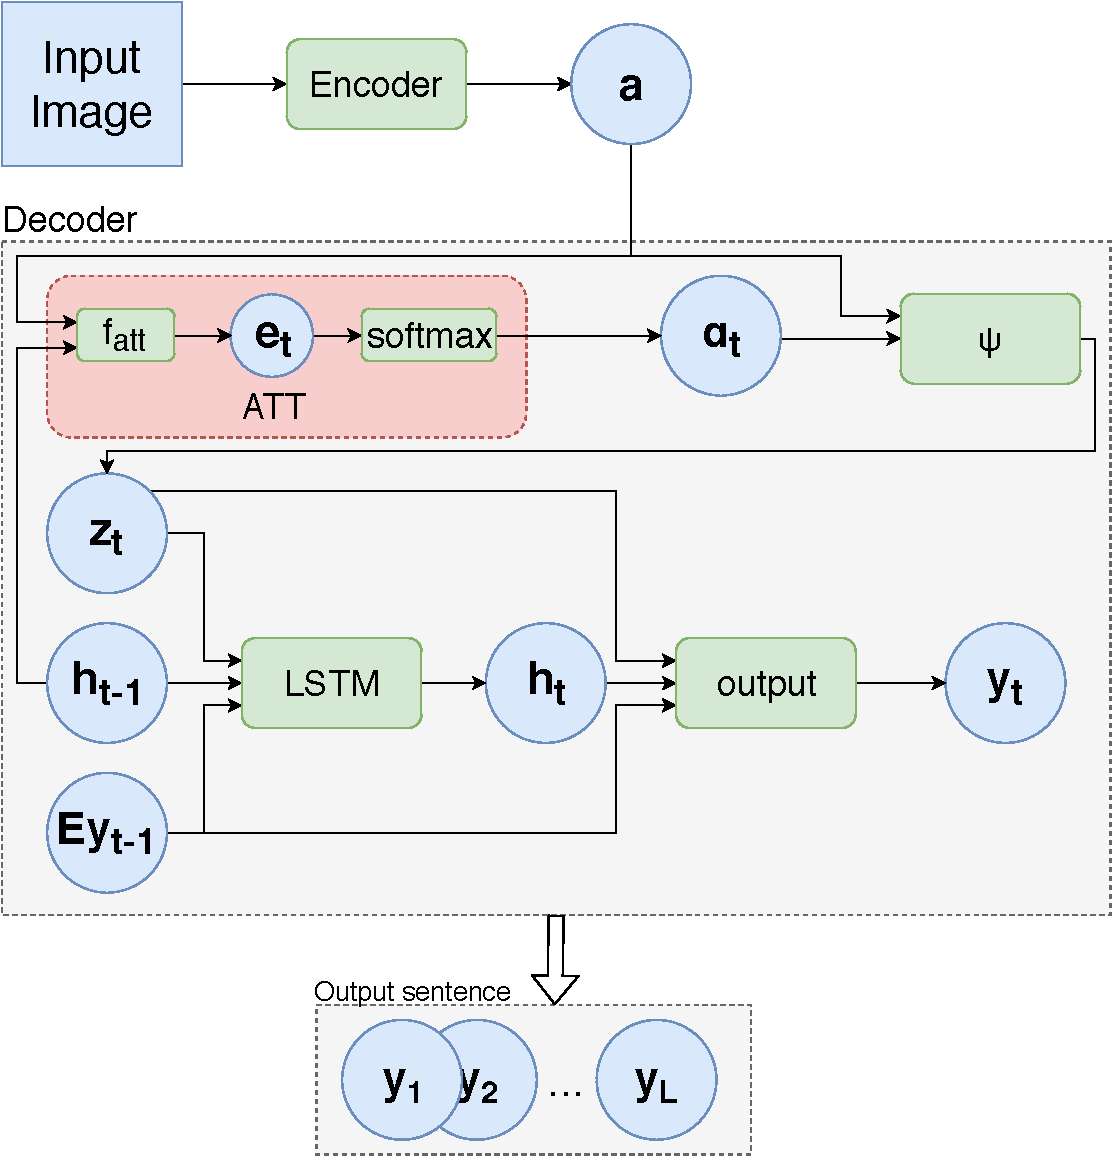
\includegraphics[width=0.7\linewidth]{./img/captioning.pdf}\label{fig:captioning}
    \caption{Model proposed for image captioning in~\cite{ref:show-attend-tell} with attentional module.}
\end{figure}

Figure~\ref{fig:captioning} illustrates the model proposed in the work.
The steps that calculate the attention to each encoding vector can be ``encapsulated'' as
an attentional module under our modeling:
$a$, the input image encoding, is the \emph{focus target input} $\tau_t$,
$h_{t-1}$, the hidden state of the model LSTM, is the \emph{outer state input} $o_t$
and $\alpha_t$, the weights given to each encoding vector, is the \emph{focus output}. In this case, $A = [0, 1]$.
Note that, in this case, the \emph{internal state} is empty.

\subsection{Adaptive Computation Time}
The work~\cite{ref:act} proposes an RNN that can perform a variable number of computation ``sub-steps'' for each time step $t'$.
The main idea is to calculate an amount $0 \le p_{t',t} \le 1$ to be ``spend'' for each computation sub-step $t$ up until the
moment the total spent reaches the ``budget'' of $1$ (in which moment the computation is halted).
The final value $y_{t'}$ is computed as an weighted average of the intermediate $y_{t',t}$ values and the weights are the values
$p_{t',t}$.

\begin{figure}[H]
    \centering
    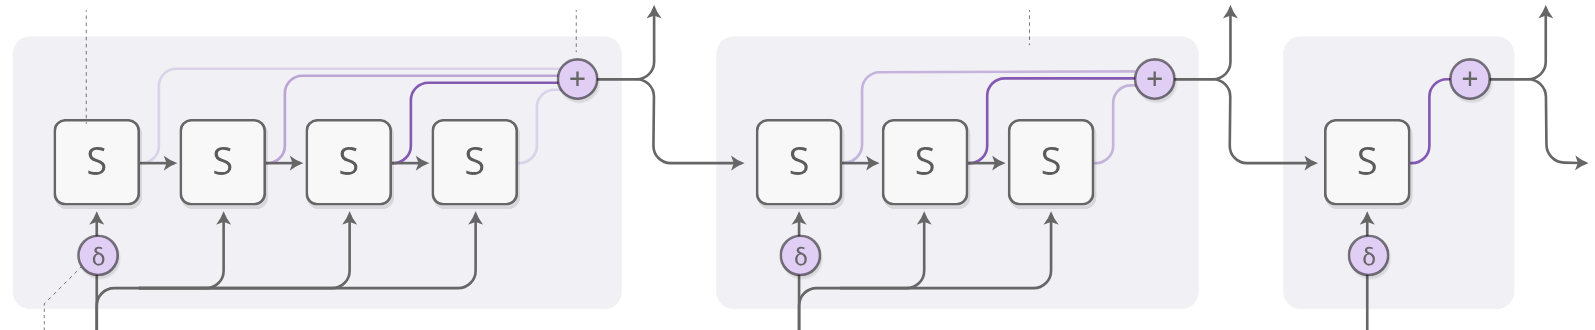
\includegraphics[width=0.8\linewidth]{./img/adaptive_comp.png}\label{fig:act}
    \caption{Adaptive computation time process illustration.}
\end{figure}

The attention component provides two types of focus:
The selection of computing substeps at each step can be thought as a focus flow with \emph{hard} continuity, \emph{enduring}/\emph{oriented} signature and \emph{computing} as focus target.
The computation of the result of each step uses \emph{soft} focus of \emph{ephemeral} signature and \emph{data} as focus target.

\begin{figure}[H]
    \centering
    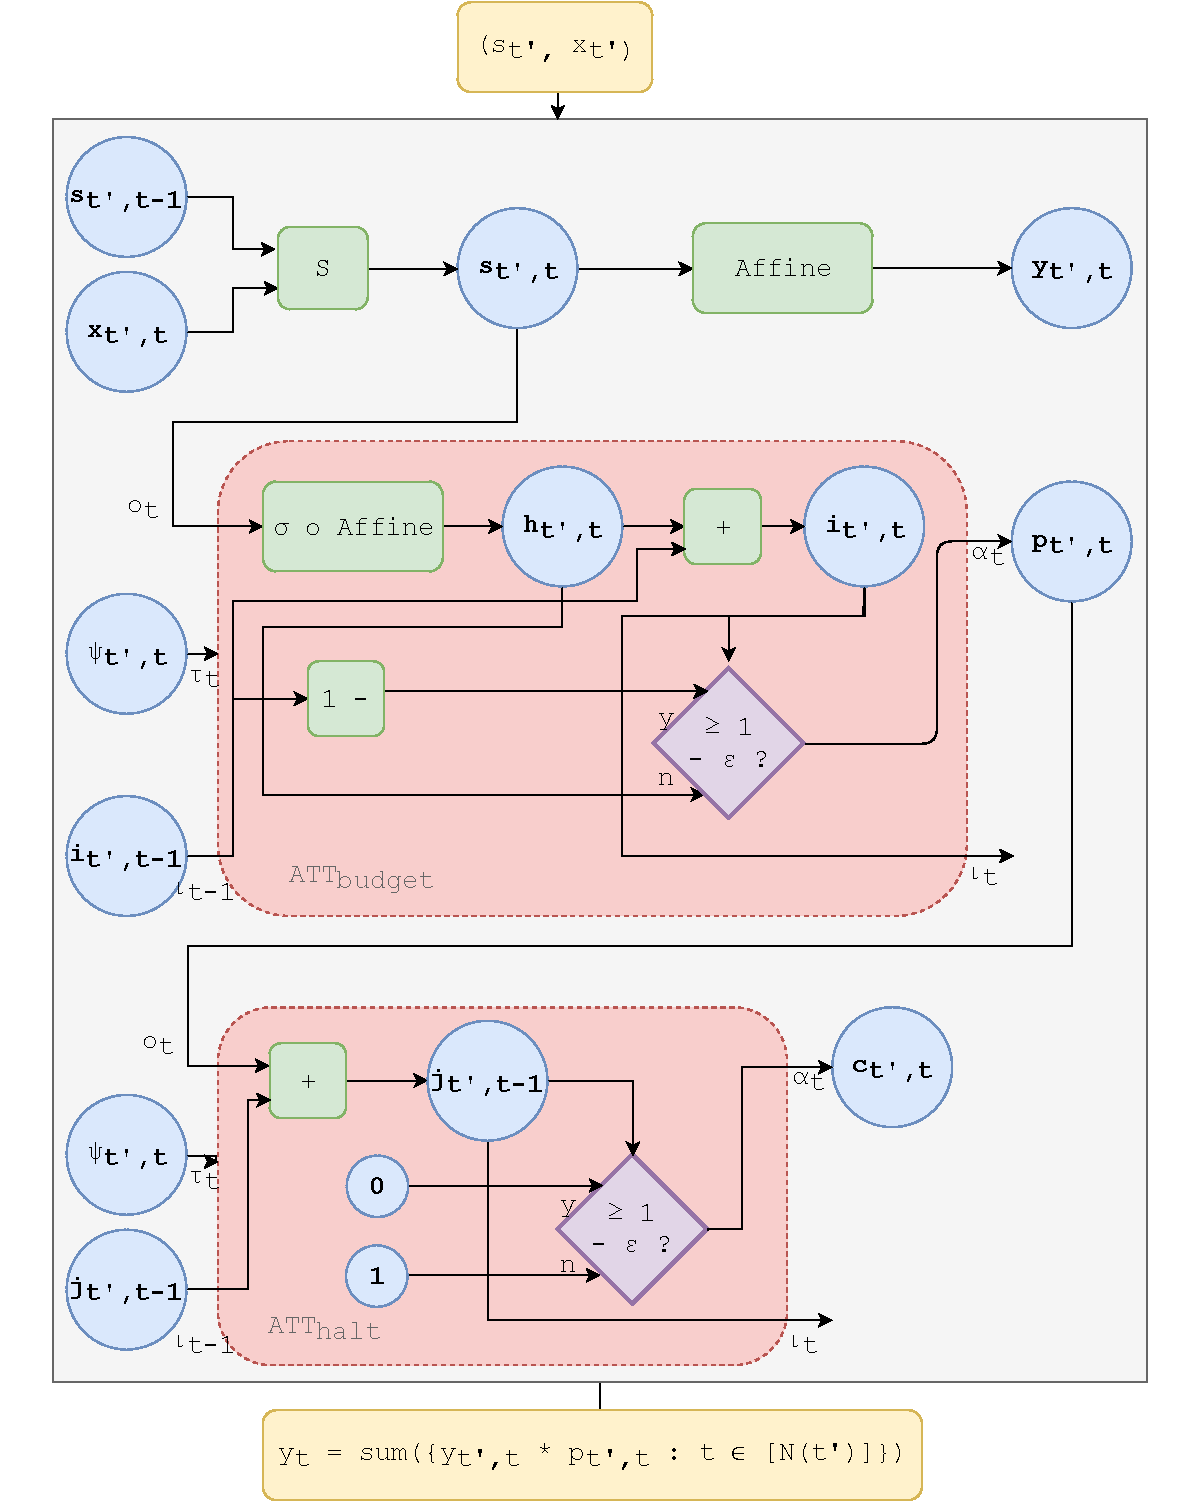
\includegraphics[width=0.65\linewidth]{./img/act.pdf}\label{fig:act}
    \caption{Model proposed for image captioning in~\cite{ref:act} with attentional module.}
\end{figure}

Figure~\ref{fig:act} illustrates the model proposed in the work.
The proposed model can be thought as having two attention modules:
\begin{itemize}
    \item \textbf{$ATT_{budget}$}, which computes the value $0 \le p_{t',t} \le 1$ to be spent at a given sub-step.
        In this analogy, $s_{t',t}$ --- the state of the RNN cell --- is the \emph{outer state} $o_t$;
        $\psi_t$ --- a dummy element representing the current computation sub-step --- is the \emph{target} $\tau_t$;
        and $i_{t',t}$ is the \emph{inner state}.
        The \emph{focus output} $p_{t',t}$, besides representing values to be consumed from the budget,
        can be thought of as an importance weight for the final output $y_t$, since the produced values are used to computed
        the weighted average.
    \item \textbf{$ATT_{halt}$}, which computes the value $c_{t',t} \in \{0, 1\}$, which is $1$ if the cell should continue
        further sub-steps and $0$ otherwise.
        In this analogy, $p_{t',t}$ is the \emph{outer state} $o_t$;
        $\psi_t$ --- a dummy element representing the current computation sub-step --- is the \emph{target} $\tau_t$;
        and $j_{t',t}$ is the \emph{inner state}.
\end{itemize}

\subsection{Recurrent Attention Model of Visual Attention}
The work~\cite{ref:ram} proposes a general recurrent model that uses visual attention at each step
by selecting a ``retina-like'' representation of a portion of the input image to carry out further computations.
At each time step $t$, the model uses the selected location $l_{t-1}$ to extract a retina-like representation
from input image.
An arbitrary action $a_t$ can be executed to possibly alter the environment.

\begin{figure}[H]
    \centering
    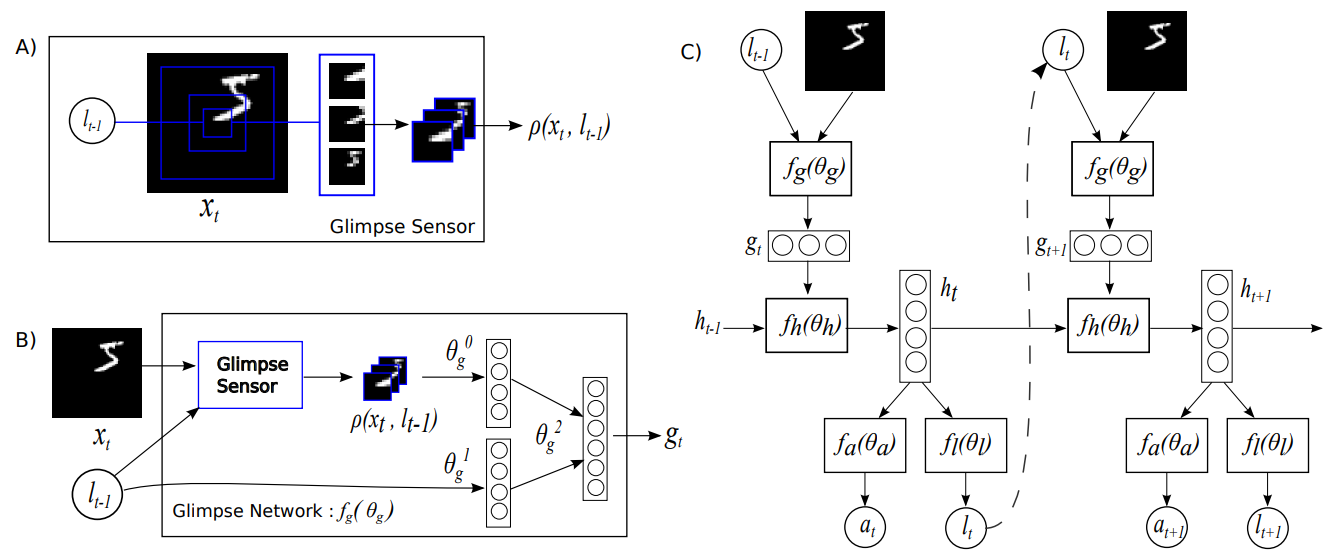
\includegraphics[width=1.0\linewidth]{./img/ram.png}
    \caption{General recurrent architecture proposed in~\cite{ref:ram}.}
\end{figure}

The attention component in the proposed model can be thought as providing
\emph{hard}, \emph{enduring}/\emph{oriented} focus to \emph{data} in a \emph{location-based} manner.

\begin{figure}[H]
    \centering
    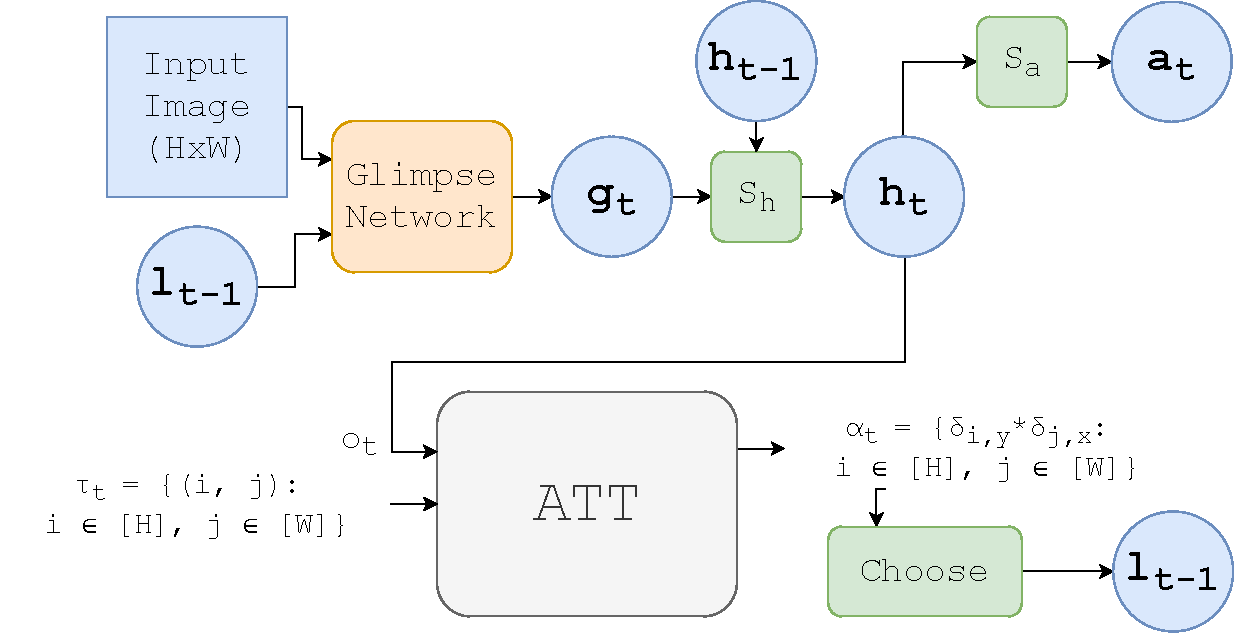
\includegraphics[width=0.7\linewidth]{./img/ram.pdf}\label{fig:ram}
    \caption{General recurrent architecture proposed in~\cite{ref:ram} with attentional module.}
\end{figure}

Figure~\ref{fig:ram} illustrates the model proposed in the work.
In this representation, the hidden state of the RNN $h_t$ is the \emph{outer state} input $o_t$;
The set of possible pixel coordinates $\{(i, j): i \in [H], j \in [W]\}$ (with $H, W$ as the height, width of the image)
is the \emph{focus targets} input $\tau_t$;
and the set $\{\delta_{i, y}\delta_{j, x}: i \in [H], j \in [W]\}$ is the \emph{focus output}.
Note that only the element $\delta_{i, y}\delta_{j,x}$ --- which is respective to the chosen pixel coordinates $(x, y)$
is equal to $1$.

Table~\ref{tab:tx} summarizes the taxonomy of the works cited above.
\begin{table}[H]
\centering
\caption{\small Taxonomy of cited works.}
    \begin{tabular}{|c|c|c|c|}
	\hline
     Work & Focus continuity & Focus flow & Focus subject\\
    \hline~\cite{ref:show-attend-tell} & Soft & Enduring/Oriented & Data\\
    \hline~\cite{ref:act} & Hard & Enduring/Oriented & Computation\\
    \hline~\cite{ref:act} & Soft & Ephemeral & Data\\
    \hline~\cite{ref:ram} & Hard & Enduring/Oriented & Data/Location-based\\
    \hline
\end{tabular}
\label{tab:tx}
\end{table}

\printbibliography\end{document}
